From Fig. 7.21 in the textbook, $\varepsilon=2k_{b}T$ and $\Delta\varepsilon=0;-2k_{b};$ and $-4k_{b}T.$\\
The grand partition function is:
\begin{align*}
Z=1+2e^{(-\beta(\varepsilon_{T}-\mu)}+e^{(-\beta(2\varepsilon_{T}-2\mu)}
+e^{-\beta\varepsilon}(1+2e^{-\beta(\varepsilon_{R}-\mu)})+e^{-\beta(2\varepsilon_{R}-2\mu)}
\end{align*}
Rearranging to group terms by ligand molecules bound,
\begin{align}
Z =[1+e^{-\beta\varepsilon}]
+[2e^{-\beta(\varepsilon_{T}-\mu})+2e^{-\beta(\varepsilon+\varepsilon_{R}-\mu)}]
+[e^{-\beta(2\varepsilon_{T}-2\mu})+e^{-\beta(\varepsilon+2\varepsilon_{R}-2\mu)}]
\end{align}
Writing expressions for $p_{0}$, $p_{1}$ and $p_{2}$,
\begin{align}
&   p_{0}=\frac{1+e^{-\beta\varepsilon}}{Z}\\
&   p_{1}=\frac{2e^{-\beta(\varepsilon_{T}-\mu)}+2e^{-\beta(\varepsilon+\varepsilon_{R}-\mu)}}{Z}\\
&   p_{2}=\frac{e^{-\beta(2\varepsilon_{T}-2\mu)}+e^{-\beta(\varepsilon+2\varepsilon_{R}-2\mu)}}{Z}
\end{align}
Let $\Delta\varepsilon=\varepsilon_{R}-\varepsilon_{T}$, such that $\varepsilon_{R}=\Delta\varepsilon+\varepsilon_{T}$.
Substituting $\varepsilon_{R}=\Delta\varepsilon+\varepsilon_{T}$ into (1),
\begin{equation}
    Z=1+e^{-\beta\varepsilon}
    +2e^{-\beta(\varepsilon_{T}-\mu})+2e^{-\beta(\varepsilon+\Delta\varepsilon+\varepsilon_{T}-\mu)}
    +e^{-\beta(2\varepsilon_{T}-2\mu})+e^{-\beta(\varepsilon+2\Delta\varepsilon+2\varepsilon_{T}-2\mu)}
\end{equation}
Similarly, substituting $\varepsilon_{R}=\Delta\varepsilon+\varepsilon_{T}$ into (2)-(4),
\begin{align}
    p_{0}&=\frac{1+e^{-\beta\varepsilon}}{Z}\\
    p_{1}&=\frac{2e^{-\beta(\varepsilon_{T}-\mu)}+2e^{-\beta(\varepsilon+\Delta\varepsilon+\varepsilon_{T}-\mu)}}
    {Z}\\
    p_{2}&=\frac{e^{-\beta(2\varepsilon_{T}-2\mu})+e^{-\beta(\varepsilon+2\Delta\varepsilon+2\varepsilon_{T}-2\mu)}}{Z}
\end{align}
Let $x =\frac{c}{c_{0}}e^{-\beta(\varepsilon_{t}-\mu_{0})}$. Rewriting (5)-(8) in terms of $x$,
\begin{align}
    Z&=1+e^{-\beta\varepsilon}
    +2x(1+e^{-\beta(\varepsilon+\Delta\varepsilon)})
    +x^{2}(1+e^{-\beta(\varepsilon+2\Delta\varepsilon)})\\
    p_{0}&=\frac{1+e^{-\beta\varepsilon}}{Z}\\
    p_{1}&=\frac{2x(1+e^{-\beta(\varepsilon+\Delta\varepsilon)})}{Z}\\
    p_{2}&=\frac{x^{2}(1+e^{-\beta(\varepsilon+2\Delta\varepsilon)})}{Z}
\end{align}
By definition, $\beta=\frac{1}{k_{b}T}$. From the question, $\varepsilon=2k_{b}T=2\beta^{-1}$. Substituting $\beta,\varepsilon$ into (9)-(12), 
\begin{align}
    Z&=1+e^{-2}
    +2x(1+e^{-(2+\frac{\Delta\varepsilon}{k_{b}T})})
    +x^{2}(1+e^{-(2+\frac{2\Delta\varepsilon}{k_{b}T})})\\
    p_{0}&=\frac{1+e^{-2}}{Z}\\
    p_{1}&=\frac{2x(1+e^{-(2+\frac{\Delta\varepsilon}{k_{b}T})})}{Z}\\
    p_{2}&=\frac{x^{2}(1+e^{-(2+\frac{2\Delta\varepsilon}{k_{b}T})})}{Z}
\end{align}
  \begin{figure}[h!]
\centering
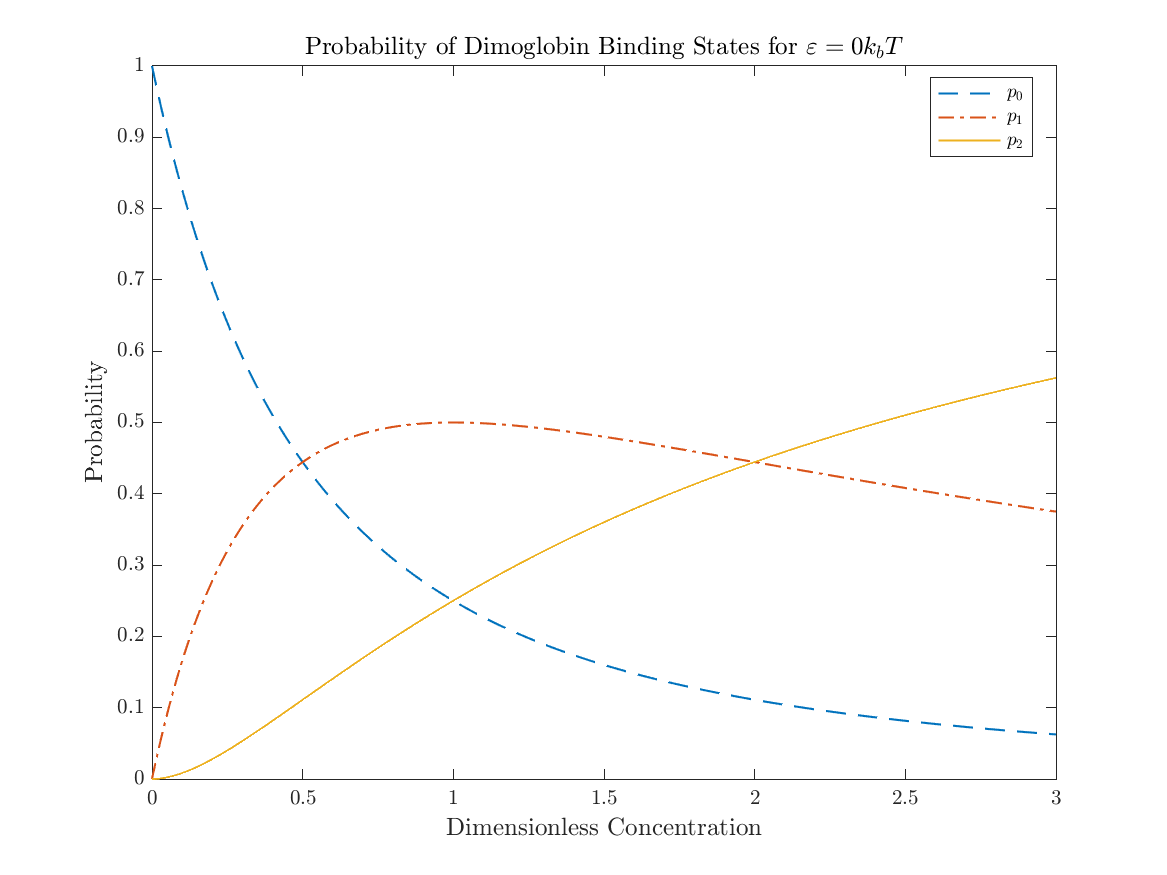
\includegraphics[height=0.46\textheight]{PHYS319_HW3_Q2_FIG0.png}
\end{figure}
\begin{figure}[h!]
\centering
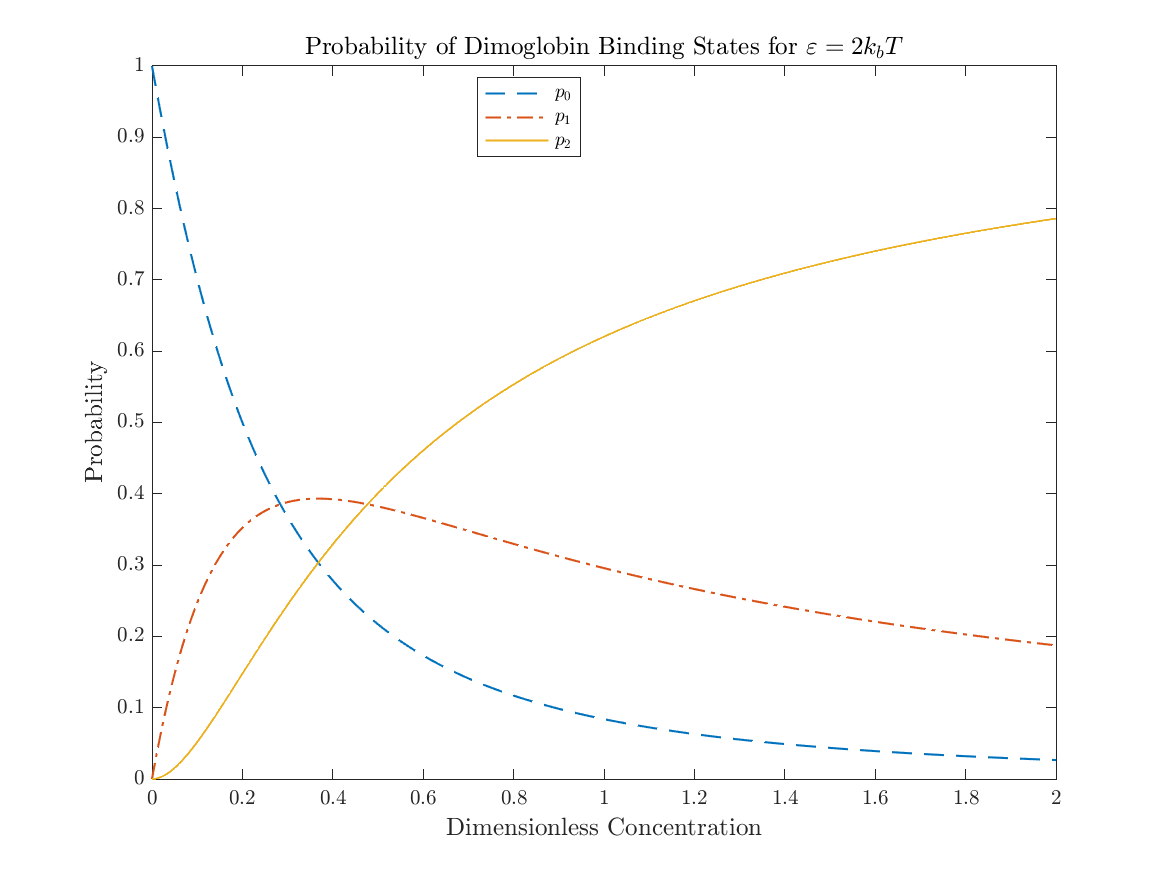
\includegraphics[height=0.48\textheight]{PHYS319_HW3_Q2_FIG2.png}
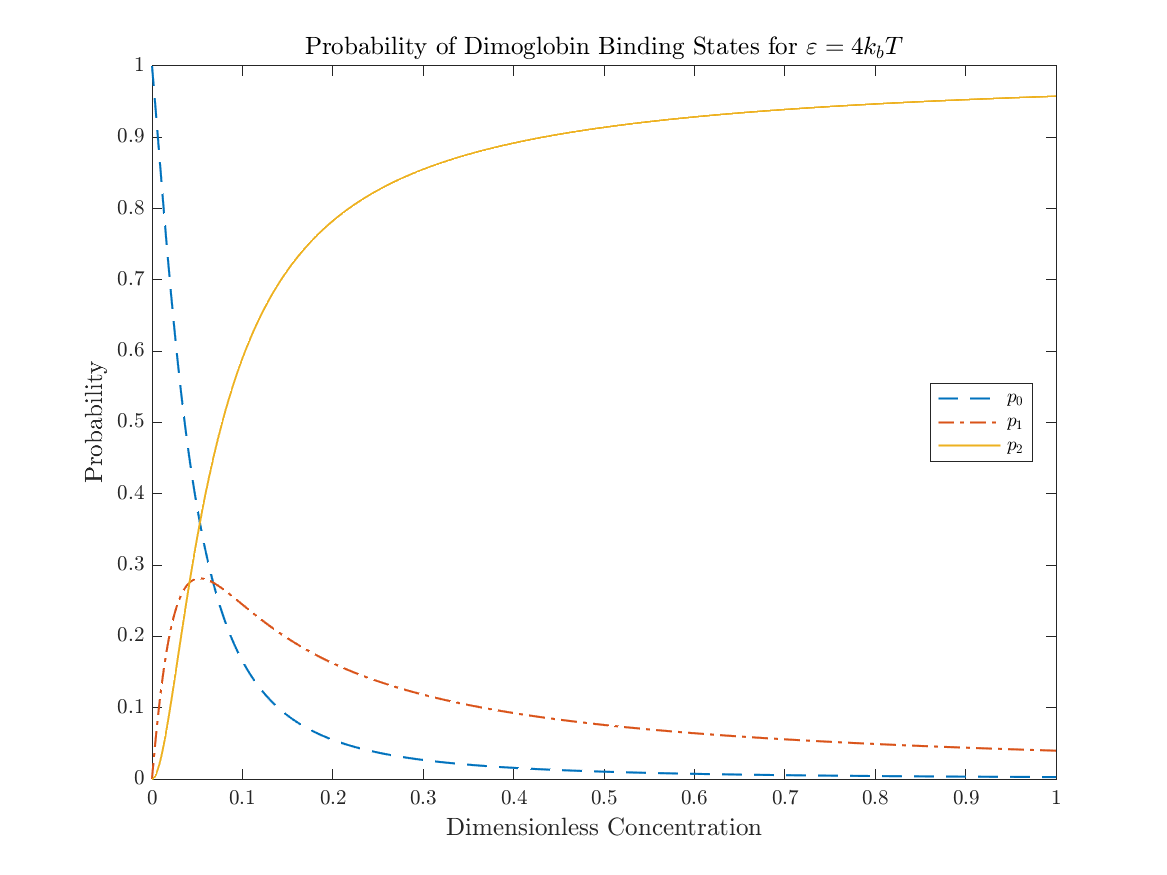
\includegraphics[height=0.48\textheight]{PHYS319_HW3_Q2_FIG4.png}
\end{figure}
